%% ============================================================================
%% main_ru.tex — русская версия. Компилировать XeLaTeX-движком (Tectonic/xelatex):
%%   tectonic -X compile main_ru.tex
%% Кириллица: libertinus-otf (Libertinus Serif) + polyglossia. Термины выверены по
%% русскоязычной лит-ре (Льюнг; Эйкхофф; Брантон-Куц, ДМК 2021).
%% ============================================================================
\documentclass[preprint,3p]{elsarticle}

\usepackage{amsmath,amssymb}
\usepackage{libertinus-otf}
\usepackage{polyglossia}
\setmainlanguage{russian}
\setotherlanguage{english}
\usepackage{microtype}
\usepackage{graphicx}
\graphicspath{{../results_scenarios/figures/}}
\usepackage{booktabs}
\usepackage[section]{placeins}   % фигуры/таблицы не выходят за свою секцию
\renewcommand{\topfraction}{0.9}
\renewcommand{\bottomfraction}{0.8}
\renewcommand{\textfraction}{0.07}
\renewcommand{\floatpagefraction}{0.75}
\setcounter{totalnumber}{5}
\journal{Computers and Electronics in Agriculture}

\begin{document}

\begin{frontmatter}

\title{Когда разреженность скрывает исполнительный механизм: предварительно
зарегистрированное экономическое сопоставительное исследование SINDy-MPC для
управления микроклиматом теплицы}

\author[a]{Автор Первый}
\author[a]{Автор Второй}
\affiliation[a]{organization={Организация, кафедра}, city={Город}, country={Страна}}

\begin{abstract}
Интерпретируемые суррогатные модели, восстановленные из данных, — в частности,
разреженная идентификация нелинейной динамики (SINDy), — привлекательны для
модельно-прогнозирующего управления (МПУ) микроклиматом теплицы, поскольку дают явные,
поддающиеся проверке уравнения, а не «чёрный ящик». Однако цену такой интерпретируемости
редко измеряют при честном протоколе: эталоны сравнения не настроены, метрикой служит
косвенный показатель слежения, а не прибыль, и — что наименее очевидно — рецепт
идентификации выбирают по качеству прогноза в разомкнутом контуре. В работе приводится
предварительно зарегистрированное вычислительное экономическое сопоставительное
исследование десяти регуляторов на имитационной модели томатной теплицы GreenLight
(Ростов-на-Дону, реальная погода ERA5 2018--2023). Первичной метрикой служит собственный
экономический показатель эффективности симулятора (EPI, сезонная прибыль), первичным
критерием — двухосевое доминирование по Парето (EPI против числа нарушений ограничений),
на 20 независимых повторах с парной непараметрической статистикой. Предварительно
зарегистрированный рецепт SINDy-MPC, замороженный по разомкнутым метрикам до какой-либо
оценки в замкнутом контуре, экономически оказывается среди слабейших интерпретируемых
регуляторов ($1{,}18$ против $4{,}63~\text{EUR/м}^2$ у настроенного эталона на правилах).
Однопараметрическая абляция вскрывает причину: порог разреженности обнуляет член котла в
уравнении температуры — единственный смоделированный орган нагрева, — и EPI в замкнутом
контуре обрушивается с $3{,}8$ до $1{,}0~\text{EUR/м}^2$, тогда как ошибка многошагового
прогноза в разомкнутом контуре остаётся почти неизменной ($2{,}25\to2{,}39$). Тем самым
критерий отбора по разомкнутому контуру нечувствителен к тому провалу замкнутого контура,
который он порождает. Восстановление члена — более плотным порогом либо методом DAgger —
возвращает EPI к паритету с эвристикой без потери интерпретируемости, а восстановленная
модель совпадает с первопринципной моделью «серого ящика». Сравнение с дополнительными
регуляторами исключает очевидные альтернативные объяснения: оракул по истинной модели
перерасходует ресурсы и не является верхней границей; нормированный PPO улучшается, но не
выигрывает; нейросетевое МПУ — худшее. Следовательно, узким местом не являются ни
недостаточная точность модели, ни интерпретируемость. Доказуемая ценность интерпретируемой
суррогатной модели лежит не в экономическом превосходстве, а в безопасности и защите при
выходе за пределы обучающего распределения. Сделан вывод: экономность модели не тождественна
её интерпретируемости; разреженность недопустимо включать в критерии отбора модели, когда
конечной задачей является управление в замкнутом контуре; предрегистрация, замороженная по
разомкнутому контуру, способна систематически удостоверять катастрофичную для управления
модель.
\end{abstract}

\begin{keyword}
управление микроклиматом теплицы \sep модельно-прогнозирующее управление \sep
разреженная идентификация нелинейной динамики \sep интерпретируемое машинное обучение \sep
идентификация для целей управления \sep экономическое сопоставительное исследование
\end{keyword}

\end{frontmatter}

%% ===========================================================================
\section{Введение}
\label{sec:intro}

Тепличное овощеводство — энергоёмкая отрасль, где решения по управлению климатом прямо
переходят в прибыль: нагрев, подкормка CO\textsubscript{2} и досветка составляют основную
долю переменных затрат, и их приходится балансировать против выручки от прироста урожая.
Модельно-прогнозирующее управление (МПУ) здесь естественно, поскольку оно оптимизирует
целевую функцию на конечном горизонте при ограничениях на температуру, влажность и
CO\textsubscript{2}, задающих продуктивный климат
\citep{vanhenten1994thesis,mayne2000constrained,lin2021greenhousempc}. Однако МПУ нуждается
в модели, а первопринципные модели теплицы трудоёмки в построении и калибровке. Это
мотивирует суррогатные модели, восстанавливаемые из данных, и в частности SINDy —
разреженную идентификацию нелинейной динамики, которая восстанавливает явные уравнения
движения как разреженную комбинацию базисных функций
\citep{brunton2016sindy,brunton2016sindyc,kaiser2018sindympc}. В отличие от нейросетевых
суррогатов, модель SINDy — «белый ящик»: её уравнения можно прочитать, проверить на
физическую и размерную согласованность и аналитически встроить в решатель МПУ. Для агронома
или сертифицирующего органа такая интерпретируемость — не роскошь, а практическое требование
доверия и отладки.

Центральный вопрос состоит в том, платят ли за интерпретируемость качеством: занимает ли
интерпретируемое SINDy-MPC недоминируемую (парето-конкурентоспособную) позицию относительно
«чёрных ящиков» или несёт измеримую «цену прозрачности». Честный ответ затрудняют три
систематических изъяна самой процедуры сравнения, распространённые в литературе по управлению
теплицами и по управлению из данных. Обученные регуляторы нередко сопоставляют с заведомо
слабой эвристикой, тогда как хорошо настроенные агрономические правила оказываются сильным
конкурентом; в качестве метрики берут ошибку слежения за уставкой вместо экономической
прибыли, хотя эти величины не связаны монотонно; наконец — и это наименее очевидно —
гиперпараметры суррогата выбирают по точности прогноза в разомкнутом контуре, молчаливо
полагая, что более точная модель даёт лучшее управление. Именно против последнего допущения три
десятилетия предостерегает идентификация для целей управления
\citep{gevers1993,vandenhof1995closedloop}, и именно его для обученной динамики заново
установило «рассогласование целевых функций» (objective mismatch)
\citep{lambert2020objective,jacobiandmd2022}.

Все три изъяна устраняются проведением предварительно зарегистрированного вычислительного
экономического сопоставительного исследования. Первичной метрикой служит собственный
экономический показатель эффективности симулятора (EPI) — сезонная прибыль, считываемая
прямо из модели вознаграждения, а не косвенный показатель. Поскольку EPI не штрафует
нарушения ограничений, первичным сравнением является двухосевое доминирование по Парето (EPI
против нарушений). Эталоны включают настроенный регулятор на правилах и честно реализованные
регуляторы обучения с подкреплением при равном бюджете гиперпараметров. Рецепт идентификации
замораживается по разомкнутым метрикам и метрикам прозрачности \emph{до} какой-либо оценки в
замкнутом контуре, следуя практике предварительной регистрации \citep{pineau2021repro},
чтобы выбор рецепта не загрязнял честное сравнение. Оцениваются десять регуляторов на 20
повторах с парной непараметрической статистикой
\citep{wilcoxon1945,holm1979,efron1994bootstrap}.

Предварительно зарегистрированная гипотеза — что SINDy-MPC недоминируемо при малой цене
прозрачности — не подтверждается. Ценность исследования, однако, не в отрицательном
результате, а в вскрытом механизме: сравнение с дополнительными регуляторами изолирует
причину недобора предрегистрированного интерпретируемого регулятора, и эта причина конкретна
и переносима на другие задачи.

Основной методологический результат работы — установленный механизм. Порог разреженности
STLSQ удаляет из модели контроль-критичный член исполнительного механизма (котла), и
экономический показатель в замкнутом контуре причинно следует за наличием этого члена, тогда
как ошибка прогноза в разомкнутом контуре к его исчезновению почти нечувствительна. Как
следствие, процедура отбора рецепта, замороженная по разомкнутому контуру ради защиты от
цикличности вывода, систематически удостоверяет модель, катастрофичную для управления, — в
чём и состоит ловушка предрегистрации. Эти наблюдения опираются на честное экономическое
сопоставление на валидированной агрономической модели, где показатель EPI поэлементно поверен
против функции вознаграждения симулятора, эталон на правилах настроен, бюджет гиперпараметров
одинаков для всех методов, а выводы подкреплены парной статистикой на двадцати повторах, —
чего недоставало прежним тепличным сравнениям, ограниченным обучением с подкреплением
\citep{vanlaatum2025greenlightgym}. Наконец, работа переосмысливает саму ценность
интерпретируемости: она проявляется в прозрачности модели, в безопасности и в способности
распознавать выход за пределы обучающего распределения, а не в экономическом превосходстве, —
и экономность описания не следует смешивать с интерпретируемостью.

%% ===========================================================================
\section{Обзор литературы}
\label{sec:related}

Оптимальное и прогнозирующее управление климатом теплицы простирается от постановки
оптимального управления связанной системой «климат--растение» у ван Хентена
\citep{vanhenten1994thesis,vanhenten2009timescale}, через современные реализации МПУ
\citep{lin2021greenhousempc,chenyou2020ddrmpc}, до стохастического оптимального управления при
погодной неопределённости \citep{vanmourik2023stochastic}. Обучение с подкреплением (ОП)
сравнивали с МПУ с неоднозначным экономическим итогом: ОП может повышать продукцию, но часто
при худшей рентабельности \citep{morcego2023rlvsmpc,mallick2024rlmpc,adaptiverobust2025greenhouse}.
Использованный здесь симулятор — GreenLight \citep{katzin2020greenlight,katzin2021led},
обёрнутый интерфейсом GreenLight-Gym \citep{vanlaatum2025greenlightgym}. Однако это
\emph{среда} для ОП: она даёт быстрый дифференцируемый симулятор и сравнивает
алгоритмы ОП, но не проводит честного экономического сравнения регуляторов с настроенным
эталоном на правилах и не рассматривает ни интерпретируемые суррогаты на разреженной
идентификации, ни вопрос об отборе по разомкнутому либо замкнутому контуру. Настоящая работа
занимает этот пробел.

SINDy восстанавливает экономные уравнения движения разреженной регрессией по библиотеке
базисных функций \citep{brunton2016sindy}, обобщается на объекты с управлением
\citep{brunton2016sindyc} и естественно сочетается с МПУ в условиях дефицита данных
\citep{kaiser2018sindympc}. Устойчивость повышают ансамблированием \citep{fasel2022ensemble},
релаксированной и ограниченной оптимизацией \citep{champion2020sr3} и зрелым инструментарием
\citep{desilva2020pysindy,kaptanoglu2022pysindy}. Базовый метод последовательного порогового
наименьших квадратов (STLSQ), однако, чувствителен к порогу разреженности: слишком большой
порог удаляет физически важные члены с малыми коэффициентами, ухудшая динамику
\citep{cortiella2021sparse,mangan2017modelselection}; на это прямо нацелены новейшие
оптимизаторы \citep{balanceguided2026}. Прежние работы трактуют это как патологию
\emph{идентификации} и предлагают лучшие \emph{оптимизаторы}; здесь же её следствие
диагностируется внутри экономического контура МПУ, с установленной причинной связью с
прибылью, и показывается, что штатный протокол отбора по разомкнутому контуру прямо в неё
попадает.

То, что точность прогноза в разомкнутом контуре — плохой косвенный показатель качества
управления в замкнутом, является фундаментальным положением идентификации для целей
управления: арбитром качества модели служит контур, а не подгонка
\citep{gevers1993,hjalmarsson1994closing,vandenhof1995closedloop,hjalmarsson2005experiment}.
Для обученной динамики это же явление заострили как «рассогласование целевых функций»:
правдоподобие одношагового прогноза не коррелирует с качеством управления
\citep{lambert2020objective,wei2023unified}, — с сопутствующими средствами в отборе,
ориентированном на ценность и на управление
\citep{farahmand2017value,controlorientedsurvey2025}. Вклад настоящей работы — не общий
принцип и не новое средство, а его конкретный, интерпретируемый и причинно проверенный
пример: поскольку суррогат является «белым ящиком», провал читается почленно (единственный
удалённый исполнительный механизм), а не диагностируется перевзвешиванием «чёрного ящика».
Для восстановления члена применяется итеративная агрегация наборов данных (DAgger)
\citep{ross2011dagger} — устоявшийся мост между экспертом-МПУ и обучаемой моделью
\citep{sun2017deeply,tagliabue2021guided,espin2024deepmpc}.

%% ===========================================================================
\section{Методы}
\label{sec:methods}

\textbf{Первичная метрика.}~Все регуляторы оцениваются по собственной экономике симулятора, а
не по косвенному показателю. На каждом шаге модель вознаграждения GreenLight возвращает
прибыль $\pi_k = g_k - c_k$, где выигрыш $g_k = (x^{\text{fruit}}_k -
x^{\text{fruit}}_{k-1})\cdot 10^{-6}/\text{dmfm}\cdot p_{\text{fruit}}$ — выручка от прироста
сухой массы плода (переводимой в сырую массу через коэффициент $\text{dmfm}=0{,}065$ и
оцениваемой по $p_{\text{fruit}}=1{,}6~\text{EUR/кг}$), а переменные затраты $c_k$ суммируют
нагрев, досветку и подкормку CO\textsubscript{2} по ценам $0{,}09$, $0{,}30$ и
$0{,}30~\text{EUR}$ за кВт·ч, кВт·ч и кг соответственно. Сезонный показатель —
$\text{EPI}=\sum_k \pi_k$ $[\text{EUR/м}^2]$. Поэлементно поверено, что пошаговая экономика,
используемая каждым регулятором (и оракулом, см. ниже), тождественна функции вознаграждения
симулятора, так что EPI — истинная целевая величина, а не приближение. Поскольку EPI не
включает штрафы за нарушения и регулятор может повышать его, чаще выходя за продуктивные
коридоры (CO\textsubscript{2} $\in[300,1600]$~ppm, $T\in[15,34]$~°C, RH $\in[50,85]\%$),
первичным сравнением служит двухосевой критерий Парето — EPI против сезонного числа шагов с
нарушениями — с указанием недоминируемого фронта (рис.~\ref{fig:pareto}). Вторичным
размерно-согласованным скаляром тяжести служит \texttt{scaled\_pen} — площадь нарушения по
каждому ограничению, нормированная по шкале самого симулятора. Единый «EPI со штрафом в евро»
не вводится, поскольку симулятор не оценивает нарушения в деньгах.

\textbf{Симулятор, локация и данные.}~Эксперименты используют модель томатной теплицы
GreenLight \citep{katzin2020greenlight} через интерфейс GreenLight-Gym
\citep{vanlaatum2025greenlightgym}. Локация — Ростов-на-Дону ($47{,}24^\circ$ с.\,ш.,
$39{,}71^\circ$ в.\,д.); реальная погода за 2018--2023~гг. взята из ERA5/ERA5-Land через
Open-Meteo, с производными членами (температура неба, почвы). Сезон — 60~суток с началом
1~марта, шаг управления 15~минут. Применяется разбиение по годам без утечки: обучение на
2018--2019, тест в пределах обучающего распределения на 2020, а 2021--2023 отложены как выход
за пределы распределения (OOD). Данные для идентификации собираются регулятором на правилах с
наложением псевдослучайного двоичного сигнала возбуждения (ПСДП, амплитуда $0{,}3$) на
исполнительные механизмы, при контроле числа обусловленности регрессии.

\textbf{Регуляторы.}~Сравниваются десять регуляторов пяти семейств
(таблица~\ref{tab:controllers}): настроенный регулятор на правилах (агрономическая эвристика —
нижний эталон и эксперт для DAgger); предлагаемое SINDy-MPC в четырёх вариантах —
предрегистрированный подтверждающий рецепт, плотный рецепт с сохранением котла и их версии,
дообученные методом DAgger; редуцированное первопринципное МПУ «серого ящика» на том же
решателе; нейросетевое МПУ (NN-MPC, суррогат $64{\times}64$); две стратегии обучения с
подкреплением, PPO \citep{schulman2017ppo} и SAC \citep{haarnoja2018sac}, через
Stable-Baselines3 \citep{raffin2021sb3}; и оракул-МПУ, планирующий по истинной динамике
симулятора. Все обучаемые регуляторы получают равный бюджет гиперпараметров (16 попыток). ОП
обучается на $2\times10^5$ шагов среды с нормировкой наблюдений и вознаграждения
(VecNormalize), пропуск которой сильно искажает результат ОП.

\begin{table*}[t]
\centering
\caption{Регуляторы и роль каждого из них в исследовании. Набор подобран так, чтобы
последовательно отвергать альтернативные объяснения недобора предрегистрированного
интерпретируемого метода.}
\label{tab:controllers}
\small
\begin{tabular}{@{}p{3.0cm}p{2.4cm}p{5.2cm}p{4.0cm}@{}}
\toprule
Регулятор & Класс & Проверяемое альтернативное объяснение & Ответ по данным \\
\midrule
На правилах & настроенная эвристика & наличие сильной простой цели (и эксперт DAgger) & да --- EPI 4,63, планка \\
МПУ «серого ящика» & редуцированная физика & слабость самих МПУ и библиотеки & нет --- 3,79 работает; причина в пороге \\
SINDy-MPC (подтверждающий) & предлагаемый, предрег. & исследуемый метод & провал: 1,18 (котёл выпал) \\
SINDy-MPC (плотный/+DAgger) & предлагаемый, починенный & устранимость дефекта без потери интерпретируемости & да --- 3,8--5,2, всё ещё «белый ящик» \\
Оракул (3\,ч, CEM) & МПУ по истинной модели & недостаток точности модели & нет --- 1,99, перерасход \\
NN-MPC & «чёрный ящик»-суррогат & преимущество «чёрного ящика» & нет --- $-5{,}09$, худший \\
PPO / SAC & «чёрный ящик»-ОП & интерпретируемость как узкое место & нет --- оба ниже эвристики \\
\bottomrule
\end{tabular}
\end{table*}

\textbf{Конвейер и предварительная регистрация.}~Предлагаемый метод проходит четыре стадии.
Сначала регулятор на правилах с наложенным ПСДП собирает данные; затем разреженная регрессия
восстанавливает интерпретируемое дискретное одношаговое отображение
$x_{k+1}=\Xi\,\Theta(x_k,u_k,d_k)$ степени~1, пригодной для аналитического встраивания в МПУ;
полученный суррогат встраивается в решатель CasADi/do-mpc, который оптимизирует согласованную с
EPI цель при климатических ограничениях на конечном горизонте; при необходимости добавляется
онлайн-адаптация (DAgger или EKF-SINDy) с монитором OOD и безопасным откатом. Рецепт идентификации (сглаживание, оптимизатор и
библиотека) не задаётся заранее: он выбирается в абляции (E2) и затем замораживается по
разомкнутым метрикам идентификации (устойчивость многошагового прогноза, встраиваемость в МПУ,
прозрачность) \emph{до} и \emph{независимо} от какого-либо EPI в замкнутом контуре на
отложенном тестовом сезоне; такая предрегистрация защищает от цикличности вывода. Замороженный
подтверждающий рецепт использует библиотеку \texttt{physics\_no\_cross}, степень~1 и
ансамблевый оптимизатор; выбранный по замкнутому контуру разведочный рецепт хранится отдельно
и приводится лишь как апостериорная чувствительность. Идентичный замороженный рецепт
загружается каждым последующим экспериментом из единого источника истины.

\textbf{Критерии допуска и статистика.}~Модель допускается к сравнению, только если проходит
критерий прозрачности (явные уравнения «белого ящика», доля пройденных проверок знаков и
размерностей выше порога, структурная устойчивость набора активных членов при бутстрепе) и
критерий встраиваемости в МПУ. Оба критерия намеренно разомкнутые; их последствия
рассматриваются ниже. Источником дисперсии служит пересбор обучающих данных на каждом повторе:
каждый повтор заново собирает набор для идентификации и переобучает суррогат, так что модели
на разных повторах действительно различаются. Используются 20~повторов для всех регуляторов;
SAC сошёлся лишь на 10~из~20 и приводится по ним. Парные сравнения проводятся критерием
знаковых рангов Уилкоксона с попарностью по повтору \citep{wilcoxon1945} и поправкой Холма
\citep{holm1979}, с указанием размера эффекта (d~Коэна) и доверительных интервалов бутстрепа
\citep{efron1994bootstrap,demsar2006}.

\textbf{Оракул.}~Оракул — регулятор на скользящем горизонте по методу кросс-энтропии (CEM),
планирующий прямо по истинному интегратору симулятора (48~выборочных последовательностей
действий, горизонт 3~часа, две итерации уточнения, «тёплый старт» от действия правил), с той
же экономической целью, что и у МПУ. Разрыв между ним и суррогатным МПУ изолирует влияние
точности модели. Верхней границей сезонного EPI оракул при этом не является: короткий
скользящий горизонт жадно максимизирует краткосрочную прибыль, а выборочный оптимизатор
деградирует на длинных горизонтах, поэтому оракул трактуется как контроль точности модели, а
не как потолок.

%% ===========================================================================
\section{Результаты}
\label{sec:results}

Десять регуляторов подобраны так, чтобы изолировать причину недобора предрегистрированного
интерпретируемого регулятора, последовательно отвергая очевидные альтернативные объяснения
(слабый МПУ, недостаточная точность модели, преимущество «чёрного ящика»). Вердикты по
предрегистрированным гипотезам сведены в таблице~\ref{tab:scorecard}.

\begin{table}[t]
\centering
\caption{Сводка по гипотезам (предрегистрированные Г1--Г4, вердикты на 20~повторах).}
\label{tab:scorecard}
\small
\begin{tabular}{@{}p{2.2cm}p{2.4cm}p{3.0cm}@{}}
\toprule
Гипотеза & Вердикт & Обоснование \\
\midrule
Центральная & не подтверждена & conf+DAgger --- ничья с правилами ($p{=}0{,}26$) \\
Г1 (разрыв до оракула) & не выполнена & оракул 1,99 $<$ правила/PPO/«серый ящик» \\
Г2 (устойчивость прогноза) & выполнена, но недостаточна & RMSE устойчив, замкнутый контур обрушивается \\
Г3 (прозрачность) & частично & бьёт NN-MPC; подтверждающий $<$ «серый ящик» \\
Г4а (адаптация) & не поддержана & DAgger $+0{,}39$, $p{=}0{,}088$; EKF хуже \\
Г4б (защита при OOD) & поддержана & защита $-50\%$ наруш., $p{\approx}10^{-24}$ \\
Г4в (без эксплуатации ошибки) & частично & подтверждающий много нарушает; защита смягчает \\
\bottomrule
\end{tabular}
\end{table}

Абляция E2 по сглаживанию, оптимизатору, библиотеке и степени (42~рецепта) выбрала — по
устойчивости многошагового прогноза и критериям прозрачности и встраиваемости — рецепт с
библиотекой \texttt{physics\_no\_cross}, степенью~1 и ансамблевым оптимизатором как
подтверждающий, замороженный до какой-либо оценки в замкнутом контуре. Расхождение
многошагового прогноза для этого рецепта пренебрежимо (доля расходящихся траекторий
$\approx 0$ при бюджете $\ge 3$~суток), так что он проходит разомкнутую планку, на которую
опирается предрегистрация. Гипотеза~\textbf{Г2} (существование рецепта с устойчивым прогнозом)
тем самым выполнена, однако, как показано ниже, устойчивости в разомкнутом контуре
необходимо, но недостаточно.

Таблица~\ref{tab:e3main} приводит EPI, нарушения и тяжесть в замкнутом контуре на 20~повторах
для всех десяти регуляторов с парной значимостью против эталона на правилах;
рисунок~\ref{fig:pareto} показывает плоскость Парето «EPI--нарушения». Вершины достигает лишь
восстановленное методом DAgger SINDy-MPC: $5{,}23\pm2{,}40~\text{EUR/м}^2$, статистически
неотличимо от $4{,}63$ у правил ($\Delta=+0{,}59$, $p_{\text{Holm}}=0{,}26$). Все остальные
регуляторы значимо хуже настроенной эвристики: МПУ «серого ящика» ($3{,}79$,
$p_{\text{Holm}}=0{,}017$), PPO ($3{,}36$, $p_{\text{Holm}}=0{,}001$), предрегистрированное
подтверждающее SINDy-MPC ($1{,}18$, $p_{\text{Holm}}=0{,}009$), SAC ($-2{,}41$) и NN-MPC
($-5{,}09$, $p_{\text{Holm}}\approx2\times10^{-5}$). Недоминируемый фронт образуют
восстановленное DAgger SINDy-MPC, эвристика на правилах, PPO и — как вырожденный угол минимума
нарушений с отрицательным EPI — SAC. По оси тяжести восстановленное DAgger SINDy-MPC
накапливает даже меньшую суммарную тяжесть нарушений, чем правила ($426$ против $485$),
несмотря на большее число шагов с нарушениями; поэтому обе оси приводятся совместно. Таким
образом, центральная предрегистрированная гипотеза не подтверждена, и единственный
интерпретируемый регулятор, дотягивающий до эвристики, достигает этого ценой починки,
механизм которой рассматривается далее.

\begin{table*}[t]
\centering
\caption{Экономическое сопоставление в замкнутом контуре (E3, 20~повторов), по убыванию EPI.
$\Delta$EPI и $p_{\text{Holm}}$ — парный критерий Уилкоксона против правил с поправкой Холма.
Фронт $=$ недоминируемость по (EPI~$\uparrow$, шаги-нарушения~$\downarrow$).}
\label{tab:e3main}
\small
\begin{tabular}{@{}lrrrrrrrc@{}}
\toprule
Регулятор & EPI & Наруш., & scaled & $T$-кор., & $n$ & $\Delta$EPI & $p_{\text{Holm}}$ & Фронт \\
 & (EUR/м$^2$) & шагов & pen & \% & & vs прав. & & \\
\midrule
SINDy-MPC (conf+DAgger) & $5{,}23\pm2{,}40$ & 4302 & 426 & 62 & 20 & $+0{,}59$ & 0,26 (нз) & $\bullet$ \\
На правилах & $4{,}63\pm0{,}00$ & 2458 & 485 & 95 & 20 & --- & --- & $\bullet$ \\
SINDy-MPC (плотный) & $3{,}81\pm1{,}27$ & 6073 & 1206 & 65 & 20 & $-0{,}82$ & 0,017 & \\
МПУ «серого ящика» & $3{,}79\pm1{,}27$ & 6083 & 1209 & 65 & 20 & $-0{,}85$ & 0,017 & \\
PPO & $3{,}36\pm1{,}59$ & 1842 & 392 & 84 & 20 & $-1{,}28$ & 0,001 & $\bullet$ \\
SINDy-MPC (плотный+DAgger) & $3{,}23\pm2{,}21$ & 4467 & 624 & 66 & 20 & $-1{,}40$ & 0,031 & \\
Оракул (3\,ч, CEM) & $1{,}99\pm0{,}68$ & 2816 & 379 & 72 & 20 & $-2{,}65$ & 2e{-}5 & \\
SINDy-MPC (подтверждающий) & $1{,}18\pm4{,}33$ & 5357 & 793 & 50 & 20 & $-3{,}46$ & 0,009 & \\
SAC & $-2{,}41\pm1{,}24$ & 1683 & 179 & 82 & 10 & $-7{,}04$ & 0,010 & $\bullet$ \\
NN-MPC & $-5{,}09\pm3{,}11$ & 4368 & 767 & 70 & 20 & $-9{,}72$ & 2e{-}5 & \\
\bottomrule
\end{tabular}
\end{table*}

\begin{figure}[htbp]
\centering

\includegraphics[width=\linewidth]{e3_pareto_annotated.png}
\caption{Плоскость Парето (EPI $\times$ нарушения, 20~повторов). Недоминируемый фронт
(красный): правила, SINDy-MPC(conf+DAgger), PPO и SAC (вырожденный угол минимума нарушений).
Починенное плотное SINDy-MPC совпадает с «серым ящиком»: экономность не тождественна
интерпретируемости.}
\label{fig:pareto}
\end{figure}

\textbf{Механизм: разреженность скрывает исполнительный механизм.}~Предрегистрированный
подтверждающий рецепт экономически слабейший среди интерпретируемых регуляторов
($1{,}18\pm4{,}33$, против $4{,}63$ у правил и $3{,}79$ у МПУ «серого ящика», делящего с ним
решатель и библиотеку). При этом рецепт отбирался не за плохое управление в замкнутом контуре:
он был заморожен, до какой-либо замкнутой оценки, как наиболее экономная модель, прошедшая
разомкнутые критерии и критерий прозрачности. Тем самым рецепт, который предрегистрация
удостоверила как оптимальный по идентификации, оказывается рецептом, проваливающимся в контуре.

Причина изолируется однопараметрической абляцией. Фиксируя библиотеку
(\texttt{physics\_no\_cross}, степень~1) и МПУ, порог разреженности STLSQ $\lambda$ варьируется
по $[10^{-6},10^{-1}]$; на каждом значении для 20~повторов фиксируются число выживших
коэффициентов, знаковый коэффициент котла в уравнении температуры
$\Xi_{u_{\text{Boil}}\to T_{\text{in}}}$ (единственного смоделированного активного органа
нагрева), \emph{разомкнутая} ошибка многошагового прогноза температуры $T_{\text{in}}$ на
тестовом сезоне и \emph{замкнутый} EPI (рис.~\ref{fig:lambda}, таблица~\ref{tab:lambda}).

\begin{figure}[htbp]
\centering

\includegraphics[width=\linewidth]{e3_lambda_sweep_ablation.png}
\caption{Свип порога разреженности $\lambda$: замкнутый EPI (синий) обрушивается по мере
обнуления коэффициента котла $u_{\text{Boil}}\!\to\!T_{\text{in}}$ (зелёный), тогда как
разомкнутая ошибка прогноза (красный) остаётся плоской. Отбор модели по разомкнутому контуру
нечувствителен к провалу замкнутого.}
\label{fig:lambda}
\end{figure}

\begin{table}[t]
\centering
\caption{Свип порога разреженности $\lambda$ суррогата \texttt{physics\_no\_cross} степени~1,
20~повторов. Коэффициент котла и замкнутый EPI обрушиваются около $\lambda\!\approx\!0{,}05$,
тогда как разомкнутая ошибка прогноза остаётся плоской.}
\label{tab:lambda}
\small
\begin{tabular}{@{}rrrrr@{}}
\toprule
$\lambda$ & ненулевых & $\Xi_{u_{\text{Boil}}\to T_{\text{in}}}$ & RMSE (разомкн.) & EPI (замкн.) \\
\midrule
$10^{-6}$ & 54,0 & 0,036 & 2,25 & 3,79 \\
$10^{-3}$ & 49,9 & 0,036 & 2,25 & 3,81 \\
0,01 & 41,8 & 0,036 & 2,27 & 4,00 \\
0,02 & 38,4 & 0,035 & 2,27 & 4,67 \\
0,03 & 34,8 & 0,032 & 2,28 & 3,49 \\
0,04 & 30,8 & 0,021 & 2,37 & 1,14 \\
0,05 & 27,7 & 0,006 & 2,38 & 0,99 \\
0,10 & 20,3 & 0,000 & 2,39 & 2,49 \\
\bottomrule
\end{tabular}
\end{table}

Две величины изменяются в противоположных направлениях. С ростом $\lambda$ от $10^{-6}$ до
$0{,}1$ модель становится экономнее (число членов $54\to20$), а коэффициент котла затухает и
исчезает: $\Xi_{u_{\text{Boil}}\to T_{\text{in}}}\approx0{,}035$ при $\lambda\le0{,}02$,
$0{,}032$ при $\lambda=0{,}03$, $0{,}006$ при $\lambda=0{,}05$ и ровно $0$ при $\lambda=0{,}1$.
Замкнутый EPI отслеживает этот обвал — с пика $4{,}67$ при $\lambda=0{,}02$ до $0{,}99$ при
$\lambda=0{,}05$, ровно там, где член котла отсекается порогом. Как только в суррогате не
остаётся органа нагрева, МПУ не может планировать отопление, и в отопительно-доминированную
весну потеря велика. Разомкнутая метрика при этом почти инертна: ошибка многошагового прогноза
изменяется лишь с $2{,}25$ до $2{,}39$ (на $6\%$), пока EPI изменяется в пять раз, а член котла
исчезает вовсе. Предрегистрированный разомкнутый критерий, следовательно, нечувствителен к
провалу замкнутого контура, который сам же вызывает. Это конкретный, физически читаемый пример
рассогласования между точностью прогноза и качеством управления
\citep{lambert2020objective,jacobiandmd2022} и реализация на разреженной идентификации того
принципа идентификации для целей управления, что арбитром качества модели должен быть замкнутый
контур \citep{gevers1993,vandenhof1995closedloop}.

Если причина — удаление члена котла, то его восстановление должно возвращать качество; оба
независимых вмешательства именно это и делают (таблица~\ref{tab:e3main}). Плотный рецепт
(\texttt{stlsq}, $\lambda=10^{-3}$) сохраняет
$\Xi_{u_{\text{Boil}}\to T_{\text{in}}}\approx0{,}034$ и поднимает EPI с $1{,}18$ до $3{,}81$;
DAgger, применённый к подтверждающему рецепту, вновь вводит член через данные замкнутого
контура и поднимает EPI до $5{,}23$, неотличимо от эталона на правилах. По всем вариантам
SINDy-MPC EPI монотонен относительно наличия коэффициента котла: при
$\Xi_{u_{\text{Boil}}\to T_{\text{in}}}\neq0$ он поднимается с $\approx1$ до
$4$--$5~\text{EUR/м}^2$. Коэффициент котла служит одномерным причинным индикатором
экономической состоятельности.

Плотная починка при этом не является «чёрным ящиком»: это то же отображение «белого ящика» с
бо́льшим числом ненулевых членов, и восстановленное плотное SINDy-MPC ($3{,}81$) совпадает с
первопринципным МПУ «серого ящика» ($3{,}79$) в пределах шума (рис.~\ref{fig:pareto}). Как
только пере-разреживание устранено, интерпретируемый суррогат схлопывается в физическую модель,
которую он призван был заменить. Разреженность отняла не точность и не прозрачность, а
управляемость, обеспечиваемую единственным членом исполнительного механизма с малым модулем.
Из этого вытекают два практических следствия. Разреженность не должна быть целью отбора модели,
когда конечная задача — управление в замкнутом контуре
\citep{farahmand2017value,cortiella2021sparse,balanceguided2026}; а критерий прозрачности,
удостоверяющий модель с обнулённым ключевым исполнительным механизмом, неполон — выпадение
такого члена само по себе должно означать провал критерия.

\textbf{Точность модели не объясняет провал.}~Если бы дело было в недостаточной точности
суррогата, выигрывало бы МПУ по истинной модели. Этого не происходит: оракул даёт лишь
$1{,}99\pm0{,}68~\text{EUR/м}^2$ (таблица~\ref{tab:e3main}), ниже эвристики, вариантов с DAgger
и плотного/«серого» и PPO. Проба по горизонту (рис.~\ref{fig:oracle}) объясняет причину: EPI
падает, а не растёт с горизонтом ($+0{,}26$ при 3~ч, $+0{,}04$ при 12~ч, $-0{,}51$ при 24~ч на
14-суточном окне, где правила дают $+0{,}63$). Прирост плода и выручка растут к уровню эвристики
по мере удлинения горизонта, но затраты — главным образом на электричество и
CO\textsubscript{2} — растут быстрее, так что оракул достигает сопоставимой продукции дороже.
Это жадный перерасход из-за короткого скользящего горизонта, а не дефицит точности, поэтому
рамка «разрыва до оракула» (гипотеза~\textbf{Г1}) здесь не является осмысленным потолком. Это
структурное свойство короткогоризонтного экономического МПУ, а не ошибка эксперимента: оракул
корректно максимизирует ровно ту величину, которую вознаграждает симулятор, — но жадно и на
слишком коротком окне.

\begin{figure}[htbp]
\centering
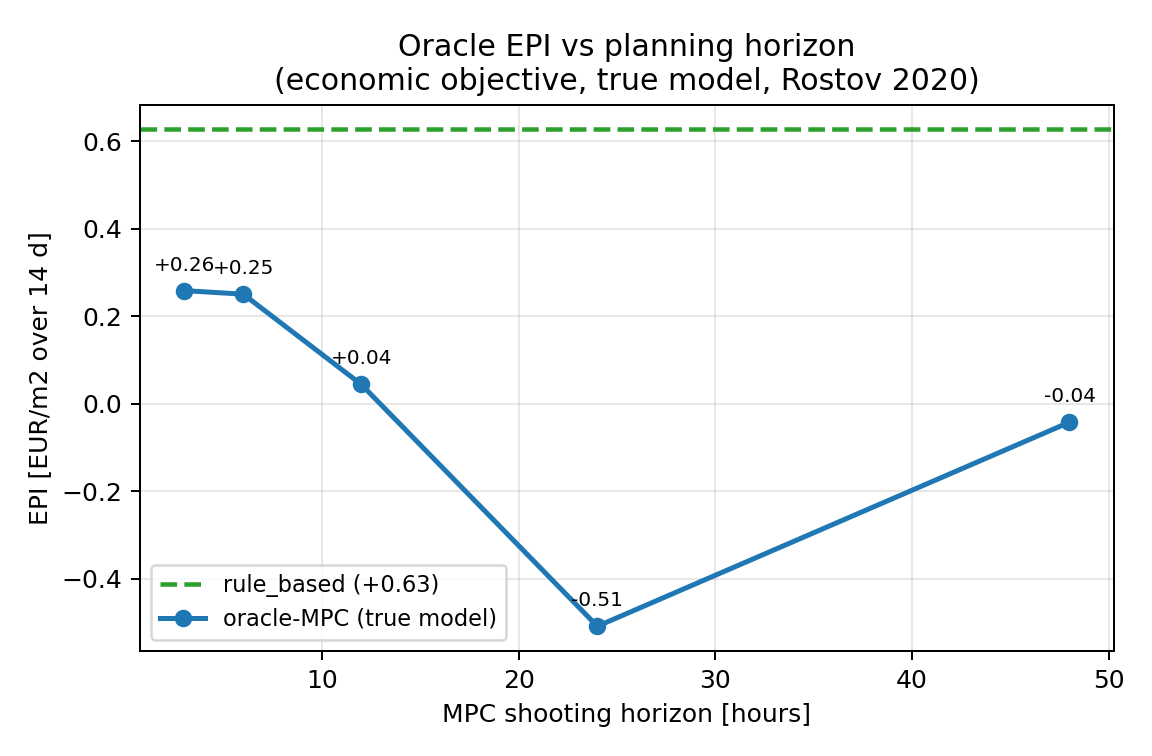
\includegraphics[width=0.82\linewidth]{oracle_horizon_sweep.png}
\caption{Оракул не является потолком. EPI экономического МПУ по истинной модели падает с
удлинением горизонта планирования и остаётся ниже эвристики на правилах (пунктир): короткий
скользящий горизонт жадно перерасходует.}
\label{fig:oracle}
\end{figure}

\textbf{Интерпретируемость не является узким местом.}~«Чёрный ящик» также не выигрывает.
Эталоны ОП чувствительны к нормировке: наивный PPO даёт $-13~\text{EUR/м}^2$, тогда как
штатная нормировка наблюдений и вознаграждения поднимает его до $+3{,}4$ — это урок
воспроизводимости, а не свойство ОП \citep{henderson2018matters}; и всё же на 20~повторах
нормированный PPO ($3{,}36$) остаётся значимо ниже эвристики, а SAC нестабилен и расходится на
10~из~20 повторов. Нейросетевое же «чёрноящичное» МПУ оказывается худшим регулятором
исследования ($-5{,}09~\text{EUR/м}^2$), проигрывая любому интерпретируемому варианту SINDy.

\textbf{Онлайн-адаптация даёт нулевой эффект.}~При весенних OOD-сдвигах (2021--2023, тот же
сезон посадки) офлайн-суррогат уже хорошо обобщается — средний EPI $\approx 0$, опережая
$-2{,}9$ у правил при том же сдвиге, — оставляя адаптации мало «зазора». На 60~парах (сдвиг
$\times$ повтор) DAgger улучшает статический офлайн-вариант лишь на $+0{,}39~\text{EUR/м}^2$
($p=0{,}088$, незначимо), а онлайн-EKF-SINDy значимо хуже ($-2{,}17$, $p<10^{-6}$); прежняя
меньшая выборка ($n=9$), намекавшая на значимый выигрыш DAgger, не выдерживает бо́льшего плана.
Гипотеза~\textbf{Г4а} не поддержана. Провал под сдвигом — не постепенный дрейф коэффициентов, а
проблема данных: в односезонных данных, собранных под сдвигом, факторы неразделимо смешаны
(корреляция $\text{corr}(u_{\text{Vent}},T_{\text{in}})=+0{,}67$ против $+0{,}03$ у многолетних
офлайн-данных), так что переобучение неверно выучивает эффект вентиляции. Устойчивость под OOD
обеспечивают структура (сохранение члена котла) и защитный монитор, а не адаптация
коэффициентов.

\textbf{Безопасность и защита при выходе за пределы распределения.}~Доказуемая ценность
прозрачного суррогата лежит в безопасности. Два его эпистемических сигнала — расстояние
Махаланобиса по экзогенным входам \citep{mahalanobis1936,lee2018mahalanobis} и дисперсия
предсказаний ансамбля \citep{lakshminarayanan2017ensembles} — коррелируют с ошибкой и прибылью
(Махаланобис: $+0{,}63$ с ошибкой прогноза, $-0{,}50$ с EPI; дисперсия ансамбля: $-0{,}57$ с
EPI), а сам сигнал служит рабочим детектором шагов с высокой ошибкой (площадь под ROC-кривой
AUC $=0{,}70$; рис.~\ref{fig:gen}). Включение защитного монитора по сигналу Махаланобиса с
откатом на регулятор правил на OOD-шагах снижает сезонные нарушения с $1723$ до $863$ (на
$50\%$), одновременно улучшая EPI (с $-2{,}06$ до $-1{,}48$); снижение высокозначимо на
200~парах ($p\approx10^{-24}$). При внесённых отказах (таблица~\ref{tab:e7},
рис.~\ref{fig:faults}) супервизор на невязках с тем же откатом значимо смягчает все шесть
типов отказов, снижая нарушения в среднем на $1304$~шага ($p\approx6\times10^{-21}$, 120~пар).
Это сильнейший положительный результат исследования (гипотеза~\textbf{Г4б}).

\begin{figure}[htbp]
\centering

\includegraphics[width=\linewidth]{e5_generalization.png}
\caption{Генерализация и детекция OOD. Слева — замкнутый EPI по парам «обучение $\to$ тест»
(зелёный — хорошо, красный — плохо). В центре — сигнал OOD (Махаланобис) коррелирует с ошибкой
прогноза ($r=0{,}63$). Справа — как детектор шагов с высокой ошибкой сигнал даёт AUC~$=0{,}70$.}
\label{fig:gen}
\end{figure}

\begin{figure}[htbp]
\centering

\includegraphics[width=\linewidth]{e7_faults.png}
\caption{Устойчивость к отказам. Шаги-нарушения при шести внесённых отказах датчиков и
механизмов без (синий) и с (оранжевый) супервизором на невязках, против бездефектного эталона
(пунктир). Супервизор значимо снижает нарушения при каждом отказе.}
\label{fig:faults}
\end{figure}

\begin{table}[t]
\centering
\caption{Внесение отказов: EPI и шаги-нарушения без и с супервизором; бездефектный эталон
EPI~$1{,}94$, нарушения~$2587$. Супервизор снижает нарушения при всех шести отказах
($p\approx6\times10^{-21}$ в целом).}
\label{tab:e7}
\small
\begin{tabular}{@{}lrrrr@{}}
\toprule
Отказ & EPI (без) & Наруш. (без) & EPI (с) & Наруш. (с) \\
\midrule
$T_{\text{in}}$ залипание & 0,86 & 4163 & 0,99 & 2055 \\
RH смещение & $-0{,}07$ & 4125 & 0,90 & 2013 \\
$u_{\text{Vent}}$ отказ & 2,01 & 3617 & 2,14 & 2558 \\
$T_{\text{in}}$ смещение & 1,62 & 3412 & 1,12 & 2165 \\
$u_{\text{Lamp}}$ отказ & 1,99 & 2574 & 2,40 & 1885 \\
$u_{\text{Boil}}$ залипание & $-3{,}18$ & 1816 & $-2{,}16$ & 1208 \\
\bottomrule
\end{tabular}
\end{table}

\textbf{Устойчивость ранжирования.}~Анализ чувствительности (рис.~\ref{fig:tornado}) показывает,
что ранжирование определяется ценами сильнее, чем проектными решениями: размах EPI от цены
плода ($19{,}7$) и цены энергии ($13{,}3~\text{EUR/м}^2$) многократно превосходит размах от
возмущения коэффициентов суррогатной модели ($2{,}7$), порога разреженности ($1{,}3$) и горизонта МПУ
($0{,}6$). Ранжирование неустойчиво к цене энергии: при дорогой энергии экономная модель
«серого ящика» обгоняет энергоёмкую эвристику. Следовательно, ранжирование по одному скаляру
ненадёжно, и предпочтительным является представление в виде структуры Парето.

\begin{figure}[htbp]
\centering

\includegraphics[width=\linewidth]{e6_sensitivity.png}
\caption{Анализ чувствительности. Размах EPI определяется ценами (плод, энергия) сильнее
проектных решений (возмущение коэффициентов суррогата, порог разреженности, горизонт); ранжирование
неустойчиво к цене энергии.}
\label{fig:tornado}
\end{figure}

%% ===========================================================================
\section{Обсуждение}
\label{sec:discussion}

\textbf{Отбор суррогата для управления.}~Центральный урок носит процедурный характер.
Предрегистрация заморозила рецепт по разомкнутым метрикам, чтобы избежать цикличности, и тем
самым выбрала модель, проваливающуюся в контуре, поскольку эта метрика нечувствительна к
следствию в замкнутом контуре. Это довод не против предрегистрации, а против предрегистрации
неверного критерия. Отсюда две поправки. Разреженность не должна входить в цели отбора модели
для управления в замкнутом контуре: член с малым коэффициентом может быть динамически
пренебрежим для прогноза, но контроль-критичен; уместны отбор, ориентированный на управление
или на ценность \citep{farahmand2017value,jacobiandmd2022}, проверка с включённым замкнутым
контуром либо оптимизаторы, защищающие малые важные члены
\citep{balanceguided2026,cortiella2021sparse}. Критерий прозрачности, в свою очередь, неполон:
критерий, удостоверяющий модель, в которой обнулён единственный орган нагрева, не проверяет
прозрачность в смысле, релевантном управлению; выпадение ключевого механизма, обнаружимое
сверкой со структурой управления, должно означать провал критерия.

\textbf{Экономность и интерпретируемость.}~Отрицательный результат можно было бы истолковать как
«цену прозрачности», однако это неверно. Починка, возвращающая качество (восстановление члена
котла), не жертвует прозрачностью: плотная модель — то же отображение «белого ящика», лишь менее
экономное. Показательно, что оно совпадает с моделью «серого ящика» в пределах шума ($3{,}81$
против $3{,}79$): как только пере-разреживание устранено, суррогат схлопывается в физическую
модель, которую замещает. Разреженность разрушила не точность и не интерпретируемость, а
управляемость. Оптимизация экономности во имя интерпретируемости способна незаметно сломать
управление.

\textbf{Сила настроенной эвристики.}~Сила эвристики и перерасход оракула имеют общий корень.
Сезонная прибыль определяется приростом плода за дни и недели, тогда как экономическое МПУ на
скользящем горизонте в несколько часов оптимизирует ближайшую прибыль и жадно урезает нагрев и
CO\textsubscript{2}, которые окупились бы позже. Хорошо настроенный набор правил неявно кодирует
те многодневные компромиссы, которых короткогоризонтный оптимизатор не видит. Продуктивный путь
к превосходству над сильными эвристиками — не лучший короткогоризонтный суррогат, а
по-настоящему длинногоризонтная экономическая постановка: терминальная функция ценности по
состоянию растения либо градиентный многодневный оптимизатор; это выделяется как ключевая
открытая проблема.

\textbf{Обобщение и ограничения.}~Механизм не специфичен для тепличного дела: любой конвейер,
который идентифицирует разреженный суррогат, выбирает разреженность по прогноз-ориентированным
критериям и встраивает его в регулятор, подвержен тому же провалу; теплица лишь делает провал
наглядным, поскольку выпавший член — именованный исполнительный механизм, чей коэффициент можно
наблюдать отслеживающим прибыль. Полученные утверждения вычислительны (in silico) и не
переносятся на физическую теплицу без отдельной валидации. Головной результат E3 использует один
тестовый сезон, поэтому у детерминированных регуляторов нулевая дисперсия по тестовой погоде, а
приводимая дисперсия отражает лишь переидентификацию суррогата; для полной характеризации
дисперсии нужно многосезонное экономическое сопоставление. Паритет с DAgger достигается ценой
дополнительного бюджета данных замкнутого контура (три итерации агрегации по пять суток). Оракул —
короткогоризонтный CEM, а не потолок. Наконец, SAC сошёлся лишь на
10~из~20 повторов и приводится как наблюдение об устойчивости, а не как настроенный конкурент.

%% ===========================================================================
\section{Заключение}
\label{sec:conclusions}

Цена интерпретируемости для МПУ на разреженной идентификации в управлении микроклиматом теплицы
измерена при протоколе, спроектированном честным: экономическая прибыль из симулятора как
метрика, настроенный эталон на правилах, честно нормированное ОП, равный бюджет гиперпараметров и
рецепт, замороженный предрегистрацией. Предрегистрированное утверждение — что SINDy-MPC
парето-конкурентоспособно при малой цене прозрачности — не подтвердилось; основной результат
состоит в вскрытом механизме. Настроенная эвристика — сильный экономический эталон, и
единственный интерпретируемый регулятор, дотягивающий до неё, достигает этого через починку,
вызванную конкретным переносимым провалом: порог STLSQ удаляет контроль-критичный член котла,
обрушивая замкнутую прибыль при неизменной разомкнутой ошибке, так что разомкнутая
предрегистрированная процедура систематически удостоверяет катастрофичную для управления модель.
Сравнение с дополнительными регуляторами исключает интуитивные альтернативы: оракул по истинной
модели перерасходует и не является потолком, нормированный PPO улучшается, но не выигрывает, а
«чёрноящичный» NN-MPC оказывается худшим. Ценность прозрачного суррогата реальна, но лежит не в
EPI: защитный монитор OOD вдвое снижает нарушения, улучшая прибыль, а супервизор отказов смягчает
шесть типов отказов. Экономность модели не тождественна её интерпретируемости, и разреженность
не входит в число целей отбора модели, когда конечной задачей является управление в замкнутом
контуре. Дальнейшая работа состоит в поиске настоящего экономического потолка —
длинногоризонтного либо терминально-ценностного регулятора, учитывающего многодневную динамику
плода, — в отборе рецепта, ориентированном на управление и защищённом от ловушки разреженности, и
в валидации «модель--реальность» (sim-to-real).

\section*{Воспроизводимость}
Все эксперименты реализованы воспроизводимыми сценариями с фиксированной инициализацией.
Публикуются реализации регуляторов, предрегистрированный замороженный рецепт, распределённые
сценарии запуска и сборки результатов для 20~повторов и анализ, порождающий каждую таблицу и
рисунок. EPI считывается из модели
вознаграждения симулятора, а его пошаговая экономика поэлементно поверена против цели оракула.

%% ===========================================================================
\bibliographystyle{elsarticle-num}
\bibliography{../../articles/references}

\end{document}
